\documentclass[a4j,twocolumn]{jsarticle}

\usepackage[top=6.6truemm,bottom=15truemm,left=9truemm,right=9truemm]{geometry}
\usepackage[dvips,dvipdfmx]{graphicx}
\usepackage{mediabb}
\usepackage{bm}
\usepackage{comment}
\usepackage{amsmath}
\usepackage{amssymb}
\usepackage{subfigure}
\renewcommand{\baselinestretch}{0.85}

\title{Over-smoothing 防止のための層ごとに重み付けするSummarize-GNN}
\author{情報科学専攻~猪口研究室~
47020726~矢嶋 悠太 }
\date{}

\begin{document}
\maketitle

%%%%%%%%%%%%%%%%%%%%%%%%%%%%%%%%%%%%%%%%
\section{はじめに}
\label{sec_introduction}

属性をもつ頂点と辺からなるグラフ構造は、SNSなど実世界の様々なデータを表現できる。
グラフの各頂点を高精度にクラス分類することは、SNSの各ユーザを適切なコミュニティに分類することに対応する。
近年、頂点の高精度なクラス分類のために、グラフを入力として、互いに属性が似ていたり、辺で結ばれている頂点同士が空間上の近い位置にマッピングされるように、各頂点をベクトル表現する、表現学習が注目されている。
頂点のベクトル表現が得られると、既存のクラス分類モデルにそのベクトル表現を入力するだけで、頂点のクラス分類が可能になる。
頂点のクラス分類精度を向上させる、質の高い頂点の表現を学習するために、近年は深層学習を用いた手法であるGraph~Neural~Network~(GNN)\cite{Kipf}が注目されている。

GNNは層数を適切に設定することで高い頂点の分類精度が得られる一方、より多層にすると分類精度が低下する。
GNNを多層化したときに、学習される頂点の表現の質が低下し、分類精度が落ちる現象をOver-smoothingという。
本論文はOver-smoothingの課題を解決することを目的とし、GNNを改良したモデルを提案する。


%%%%%%%%%%%%%%%%%%%%%%%%%%%%%%%%%%%%%%%%
\section{グラフの定義及び問題定義}
\label{sec_definition}

\vspace{-1mm}
グラフを$G=(V,E,X)$とする。ここで$V$は$n$個の頂点集合$\{1,\ldots,n\}$、$E$は頂点$v$から$u$への有向辺$e_{vu}$の集合である。
また、各頂点$v$がもつ属性$\bm{x}_v$は$a$次元のベクトルとし、全頂点の属性の集合を$X=\{ \bm{x}_1, \ldots, \bm{x}_n \}$とする。

頂点のクラス分類について説明する。
全頂点のクラスラベル集合を$Y=\{y_1,\ldots,y_n\}$とする。
グラフ$G$とモデルの学習に用いる教師ラベル集合$Y_{train} \subset Y$を用いて、モデルを学習する。
残りの頂点のラベル集合$Y_{test}=Y \backslash Y_{train}$を用いて、学習済みモデルの分類精度を求める。

本研究では、グラフ$G$を入力とし、全頂点のベクトル表現$H=\{\bm{h}_1, \ldots ,\bm{h}_n\}$を出力することを目的とする。
具体的には、頂点の分類精度を向上させる質の高い$H$を出力するモデルを提案する。


%%%%%%%%%%%%%%%%%%%%%%%%%%%%%%%%%%%%%%%%
\section{近傍内の頂点の属性を集約するGNN}
\label{sec_gnn}

GNNは、$G$と層数$L$を入力とし、頂点$v$の表現$\bm{h}_v$を求める。
\begin{align}
  & \bm{h}_v^l = \text{Conv}(H^{l-1}, N(v)) = \sigma\left( W^l \sum_{u\in N(v)} w_{vu}^l\bm{h}_u^{l-1} \right) \label{eq_gnn1} \\
  & \bm{h}_v   = \bm{h}_v^L \label{eq_gnn2}
\end{align}
頂点$v$自身を含む、有向辺$e_{vu}$により$v$に接続されている頂点の集合$:\{v\} \cup \{u ~|~ e_{vu} \in E\}$を「$v$の1近傍内」と呼ぶ。
また、$\bm{h}_v^0$は属性$\bm{x}_v$、$\sigma(\cdot)$は活性化関数である。
$l-1$から$l$層に進む度、式(\ref{eq_gnn1})の畳み込み$\text{Conv}$により、頂点$v$の潜在表現$\bm{h}_v^{l-1}$を$\bm{h}_v^{l}$に更新する。
各$l$層の$\text{Conv}$では以下を順に実行する。\vspace{-1mm}
\begin{itemize}
  \item[1.] $v$の1近傍内の各頂点$u\in N(v)$の表現を足し合わせる集約\vspace{+1mm}
  \item[2.] 行列$W^l$と活性化関数$\sigma(\cdot)$による線形及び非線形な変換\vspace{-1mm}
\end{itemize}
よって、Convを2回繰り返して得られる表現$\bm{h}_v^2$には、$v$の1近傍内である$u\in N(v)$の、更に1近傍内である$u' \in N(u)$の属性$\bm{x}_{u'}$が集約される。
つまり、$\bm{h}_v^2$には2近傍内の頂点$u' \in N(v,2)$の属性$\bm{x}_{u'}$が集約される。

式(\ref{eq_gnn2})より、GNNは$\text{Conv}$を層数$L$回繰り返して得られる、$L$近傍内の頂点の属性が集約された$\bm{h}_v^L$を$\bm{h}_v$として出力する。

GNNは層数$L$を適切な層数$L_v^*$に設定することで、質の高い表現を得ることができ、近年最高峰の分類精度を達成している。
一方、GNNの層数$L$を$L_v^*$より大きくする程、表現$\bm{h}_v(=\bm{h}_v^L)$の質が低下し、その後のクラス分類精度も低下する現象をOver-smoothingと呼ぶ。
適切な層数$L_v^*$のGNNが質の高い表現を得て、より多層$L(\le L_v^*)$のGNNが質の低い表現を得る理由について、本資料では、教師ラベル$Y_{train}$を用いることなく独自の観点から考察していく。

%%%%%%%%%%%%%%%%%%%%%%%%%%%%%%%%%%%%%%%%
\section{提案インターフェース:Summarize-GNN}
\label{sec_proposal}

\begin{align}
  & \bm{h}_v   = \text{Summarize}(\bm{h}_v^1,\ldots,\bm{h}_v^L) = \sum_{l=1}^L \alpha_v^l \bm{h}_v^l \label{eq_summarize1}
\end{align}
但し、$\alpha_v^l$は学習可能パラメータであり、$\sum_{l=1}^L \alpha_v^l=1$を満たす。

式(\ref{eq_gnn1})で示す従来のGNNのConvを$L$回繰り返し、表現の系列$\{\bm{h}_v^1,\ldots,\bm{h}_v^L\}$を得る。
次に、式(\ref{eq_gnn2})で示すSummarize関数に$\{\bm{h}_v^1,\ldots,\bm{h}_v^L\}$を入力し、
各表現$\bm{h}_v^l$をパラメータ$\alpha_v^l$で重み付け和して得たものを最終的な表現$\bm{h}_v$として出力する。
尚、インターフェースを説明するこの節では、$\alpha_v^l$の具体的な学習手法は述べない。

もしパラメータ$\alpha_v^l$が適切に学習できれば、頂点$v$が図\ref{fig_example}の頂点$1$については、$(\alpha_1^1,\alpha_1^2,\alpha_1^3)=(1,0,0)$で、1近傍内の属性が集約されている表現$\bm{h}_1^1$に大きな重み付けができる。
一方、図\ref{fig_example}よりも大きなグラフの端にある頂点$v$については、$(\alpha_v^1,\alpha_v^2,\alpha_v^3)=(0,0,1)$で、より遠い近傍内の属性が集約されている表現$\bm{h}_v^3$に大きな重み付けができる。
つまり、$\alpha_v^l$は、$l$が、頂点$v$にとって適切な集約距離$L_v^*$である確率と捉えられる。
また、この$\alpha_v^l$を学習することは、頂点$v$ごとに適切な集約距離$L_v^*$を学習することに対応し、Over-smoothing防止が期待できる。

%%%%%%%%%%%%%%%%%%%%%%%%%%%%%%%%%%%%%%%%
\section{提案手法:$\alpha_v^l$の教師なし学習}
\label{sec_oversmoothing}

どのような条件を満たすときに、各$\alpha_v^l$が高くなるか考える。
教師ラベルを全て用いてよい($Y_{train}=Y$)なら、$v$の$l$近傍内を、$v$と同ラベルの頂点$u$が多く占めるときの層数$l$こそが適切と考えられる。よってこの条件を満たす時$\alpha_v^l$が高くなると考えられる。

本研究では、教師ラベルを用いずに($Y_{train}=\varnothing$)、どのような条件を満たすときに各$\alpha_v^l$が高くなるか考える。
説明のため、以下の各頂点$v$が単一の属性値$x_v\in \mathbb{R}$をもつ図の例を用いる。
属性値$x_v$の大きさは、各頂点$v$の色の濃さで表す。
また、各頂点の属性$x_v$はクラスラベル$y_v$に応じたガウス分布に従うと仮定する。
例えばクラス数$c=2$のこの例の場合、クラスラベルが1の頂点の属性値$x_1,x_2,x_3$は$\mathbb{G}(\mu_1, \sigma_1^2)$に、クラスラベルが2の頂点の属性値$x_4,x_5,x_6$は$\mathbb{G}(\mu_2, \sigma_2^2)$に従う。

この仮定の下、$l(=1,2,3)$が、頂点1にとって適切な集約距離$L_1^*$である確率$\alpha_1^l$が高くなる条件を考える。

\begin{figure}[!h]
  \centering
  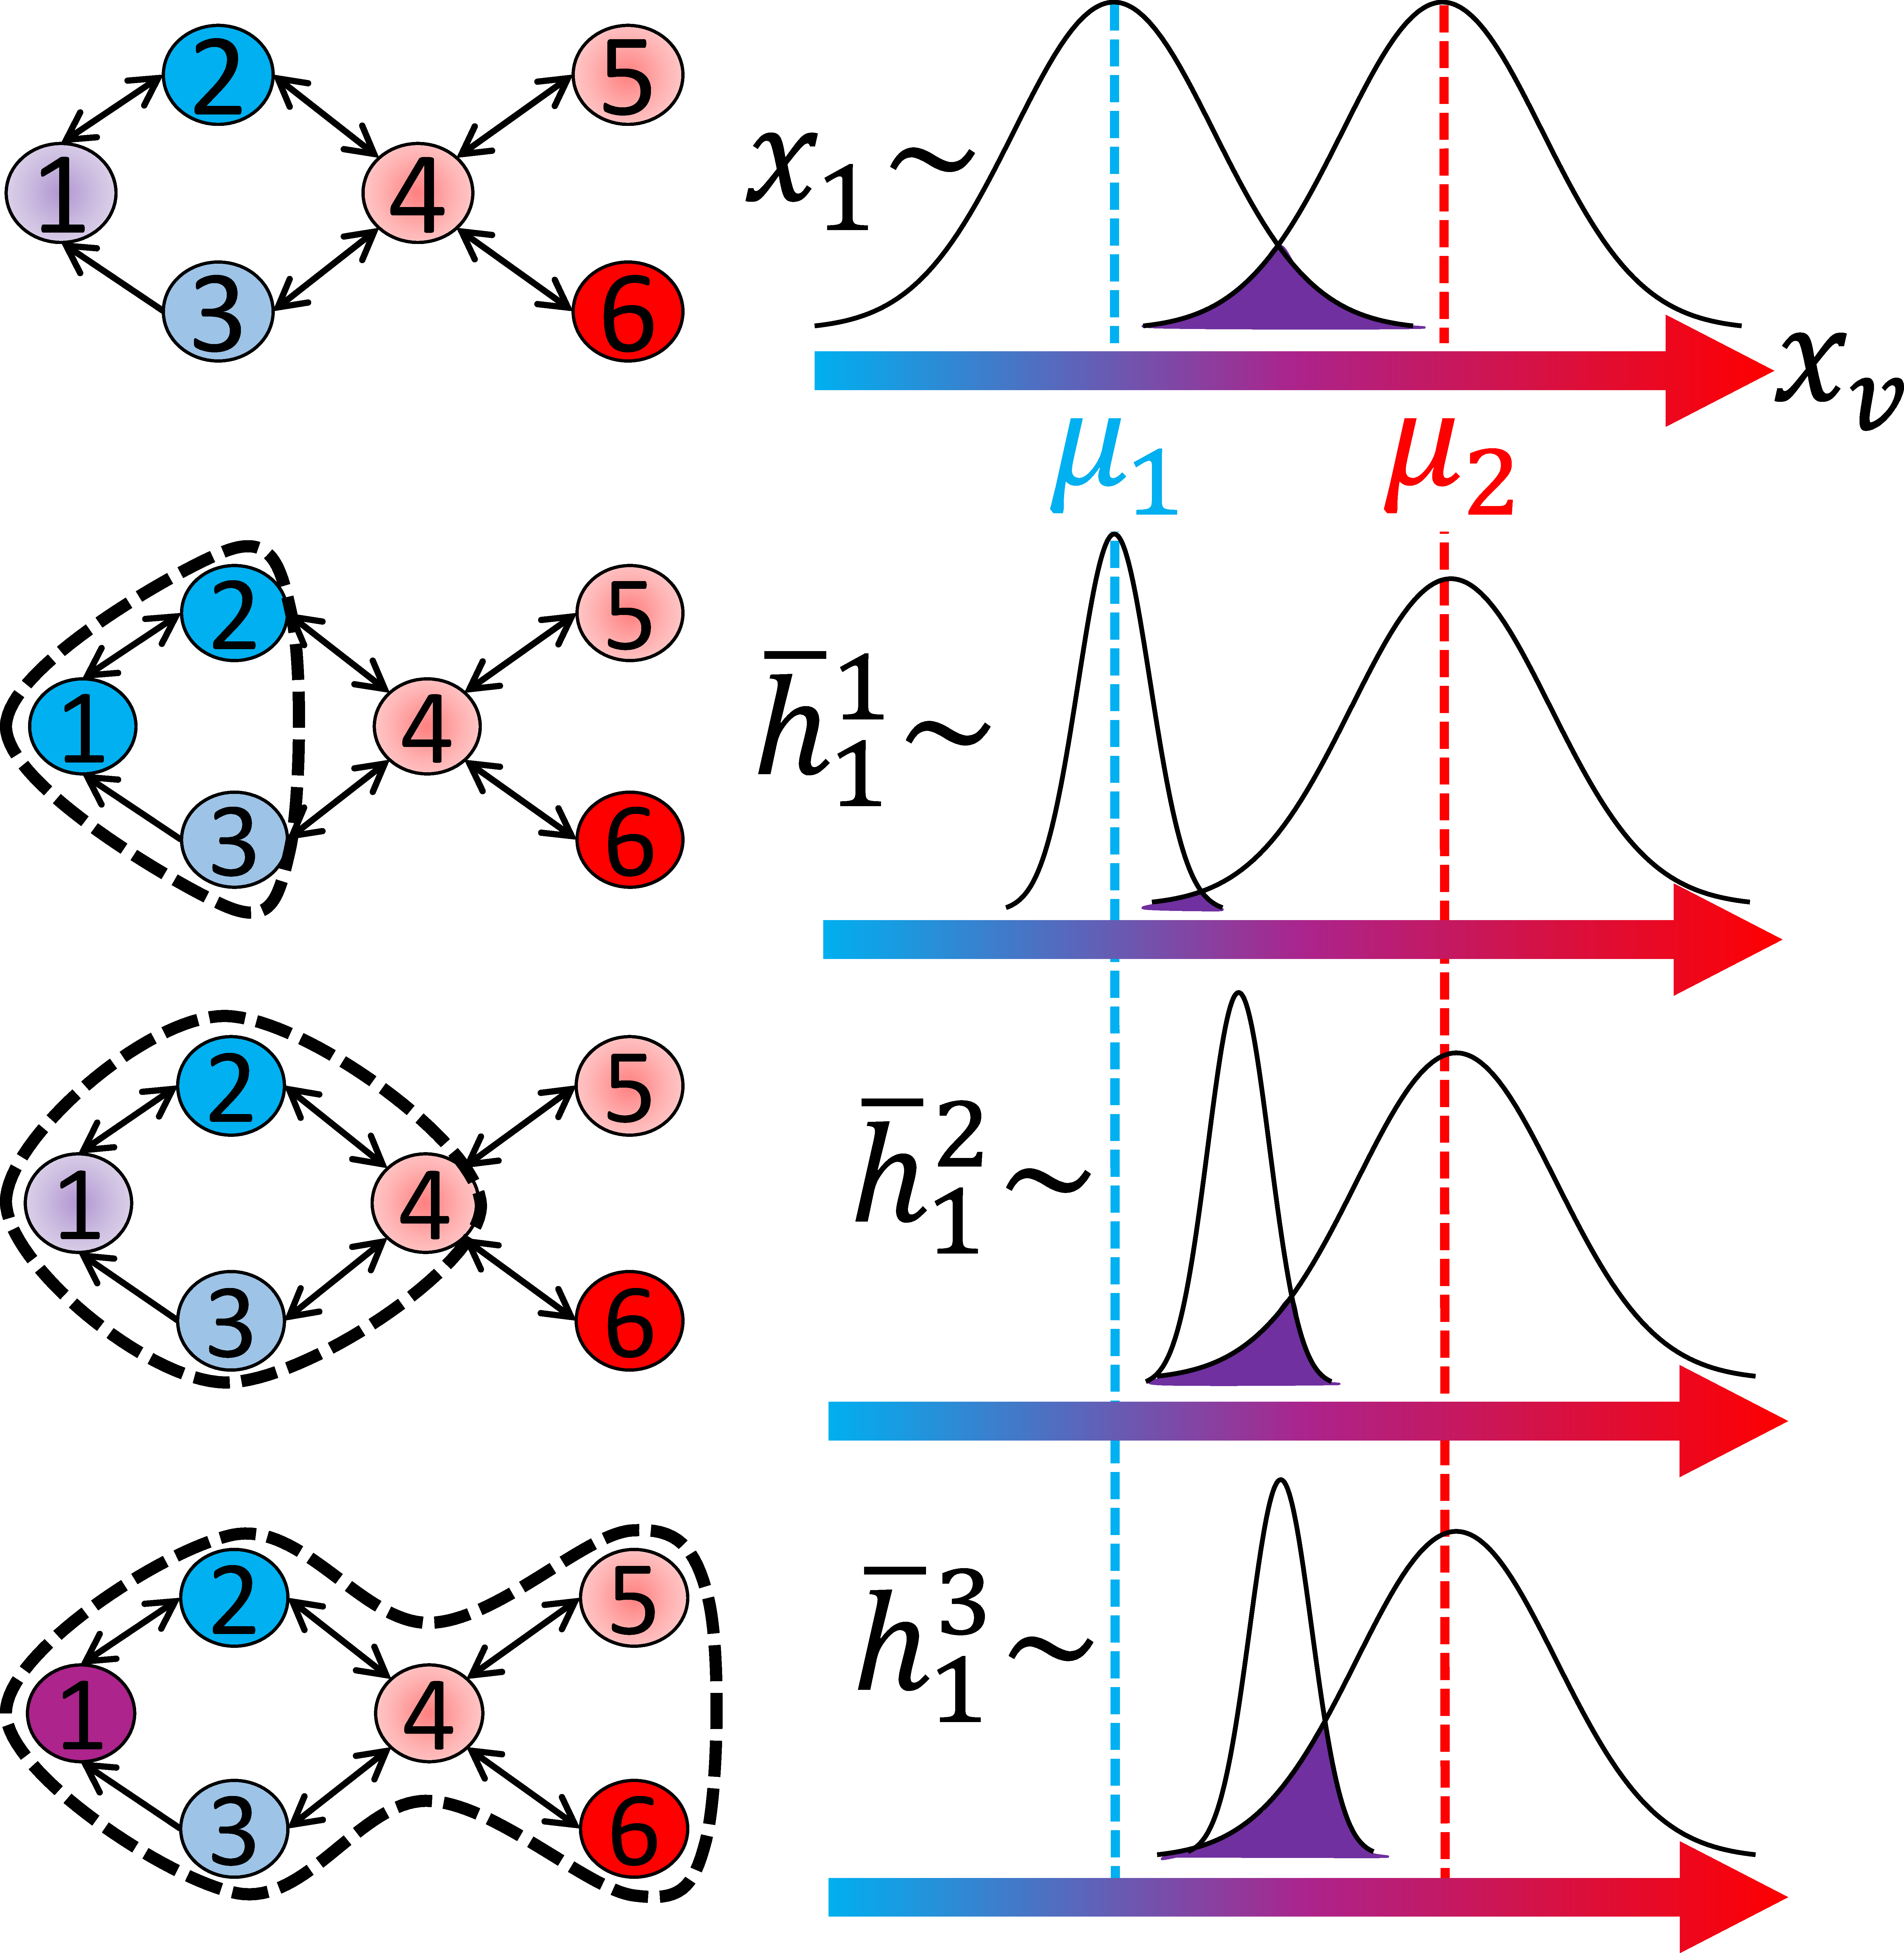
\includegraphics[height=10cm,width=9.5cm]{example.pdf}
  \vspace{-6mm}
  \caption{グラフ$G$と、集約距離$l$により変化する$h_1^l$の従う分布}
  \label{fig_example}
\end{figure}

$\mathbb{G}(\mu_1, \sigma_1^2)$と$\mathbb{G}(\mu_2, \sigma_2^2)$間には、図\ref{fig_example}右列一段目の紫色で塗りつぶした重なりがある。
図\ref{fig_example}左列で紫色で塗り分けている頂点1の属性値$x_1$は、その重なった位置から生起しているため、頂点$v$のクラスラベルが1か2を予測することは困難である。
つまり、分布間の重なりが大きくなるほど、頂点を正しくクラス分類することは困難になる。

しかし、層数1のGNNによって、頂点$1$には、1近傍内の属性が集約、足し合わされる(図\ref{fig_example}左列二段目)。
つまり、同じガウス分布$\mathbb{G}(\mu_1, \sigma_1^2)$に従う属性が足し合わされる。
同じガウス分布に従う属性を足し合わせることで得られる表現が従う分布は、元々従う分布$\mathbb{G}(\mu_1, \sigma_1^2)$と比較して、平均は維持したまま分散が小さくなる(図\ref{fig_example}右列一段目と二段目を比較)、ということが分布の再生成という統計の性質から知られている。
よって、分布間の重なりを減らすことができ、頂点$v$を正しくクラス分類することが期待できる。
また、このときの層数こそが、頂点$1$にとって適切な層数$L_1^*$と考える。

しかし、$L_1^*$を超えて、2,3層と、よりGNNを多層にすると、異なるガウス分布$\mathbb{G}_2$から生起する属性も頂点$v$に足し合わされる(図\ref{fig_example}左列三、四段目)。
すると、同じく分布の再生成という性質から、分布の平均は$\mu_1$と$\mu_2$の間にずれるため、分布間の重なりが増え、質の低い表現を得ることが危惧される(図\ref{fig_example}右列二段目から三、四段目)。
結果として、多層にする程分類精度が低下するOver-smoothingを引き起こすと考えられる。

以上から、GNNの層数$l$を1,2,3と伸ばすに連れて、各表現$\bm{h}_1^l$の従う分布がどのように移り変わるか観察した。
その上で、本研究では、多層のGNNで得られる質の低い表現と、最も類似度が低い表現$\bm{h}_v^l$が得られるときの層数$l$こそが$L_v^*$と考える。
$v$が図\ref{fig_example}のグラフの頂点1の場合の例で、説明する。
図\ref{fig_example}右列二段目の分布から生起する表現$\bm{h}_1^1$と、右列四段目の分布から生起する表現$\bm{h}_1^3$間の類似度の期待値は低い。
よって1層が$L_1^*$の確率が高いと考える。


上記で述べた$\alpha_v^l$の学習手法は以下で具体的に求める。
\begin{align}
  & \overline{\alpha}_v^l = \text{Attention}(\bm{h}_v^l, \bm{h}_v^L) \label{eq_alpha_unnormalized} \\
  & \alpha_v^l = \text{Softmax}(\overline{\alpha}_v^l, L) = \frac{\exp(\overline{\alpha}_v^l)}{\sum_{l'=1}^L \exp(\overline{\alpha}_v^{l'})} \label{eq_alpha_normalized}
\end{align}
式(\ref{eq_alpha_unnormalized})のAttentionとは、ベクトル間の関連度(類似度など)を深層学習法で解析する際に近年盛んに使われている機構である。
このAttention関数を用いて$\bm{h}_v^l$と$\bm{h}_v^L$間の類似度を求め、$\overline{\alpha}_v^l$として出力する。
式(\ref{eq_alpha_normalized})のSoftmax関数により、制約$\sum_{l=1}^L \alpha_v^l=1$を満たすように正規化する。

\begin{figure}[!h]
  \centering
  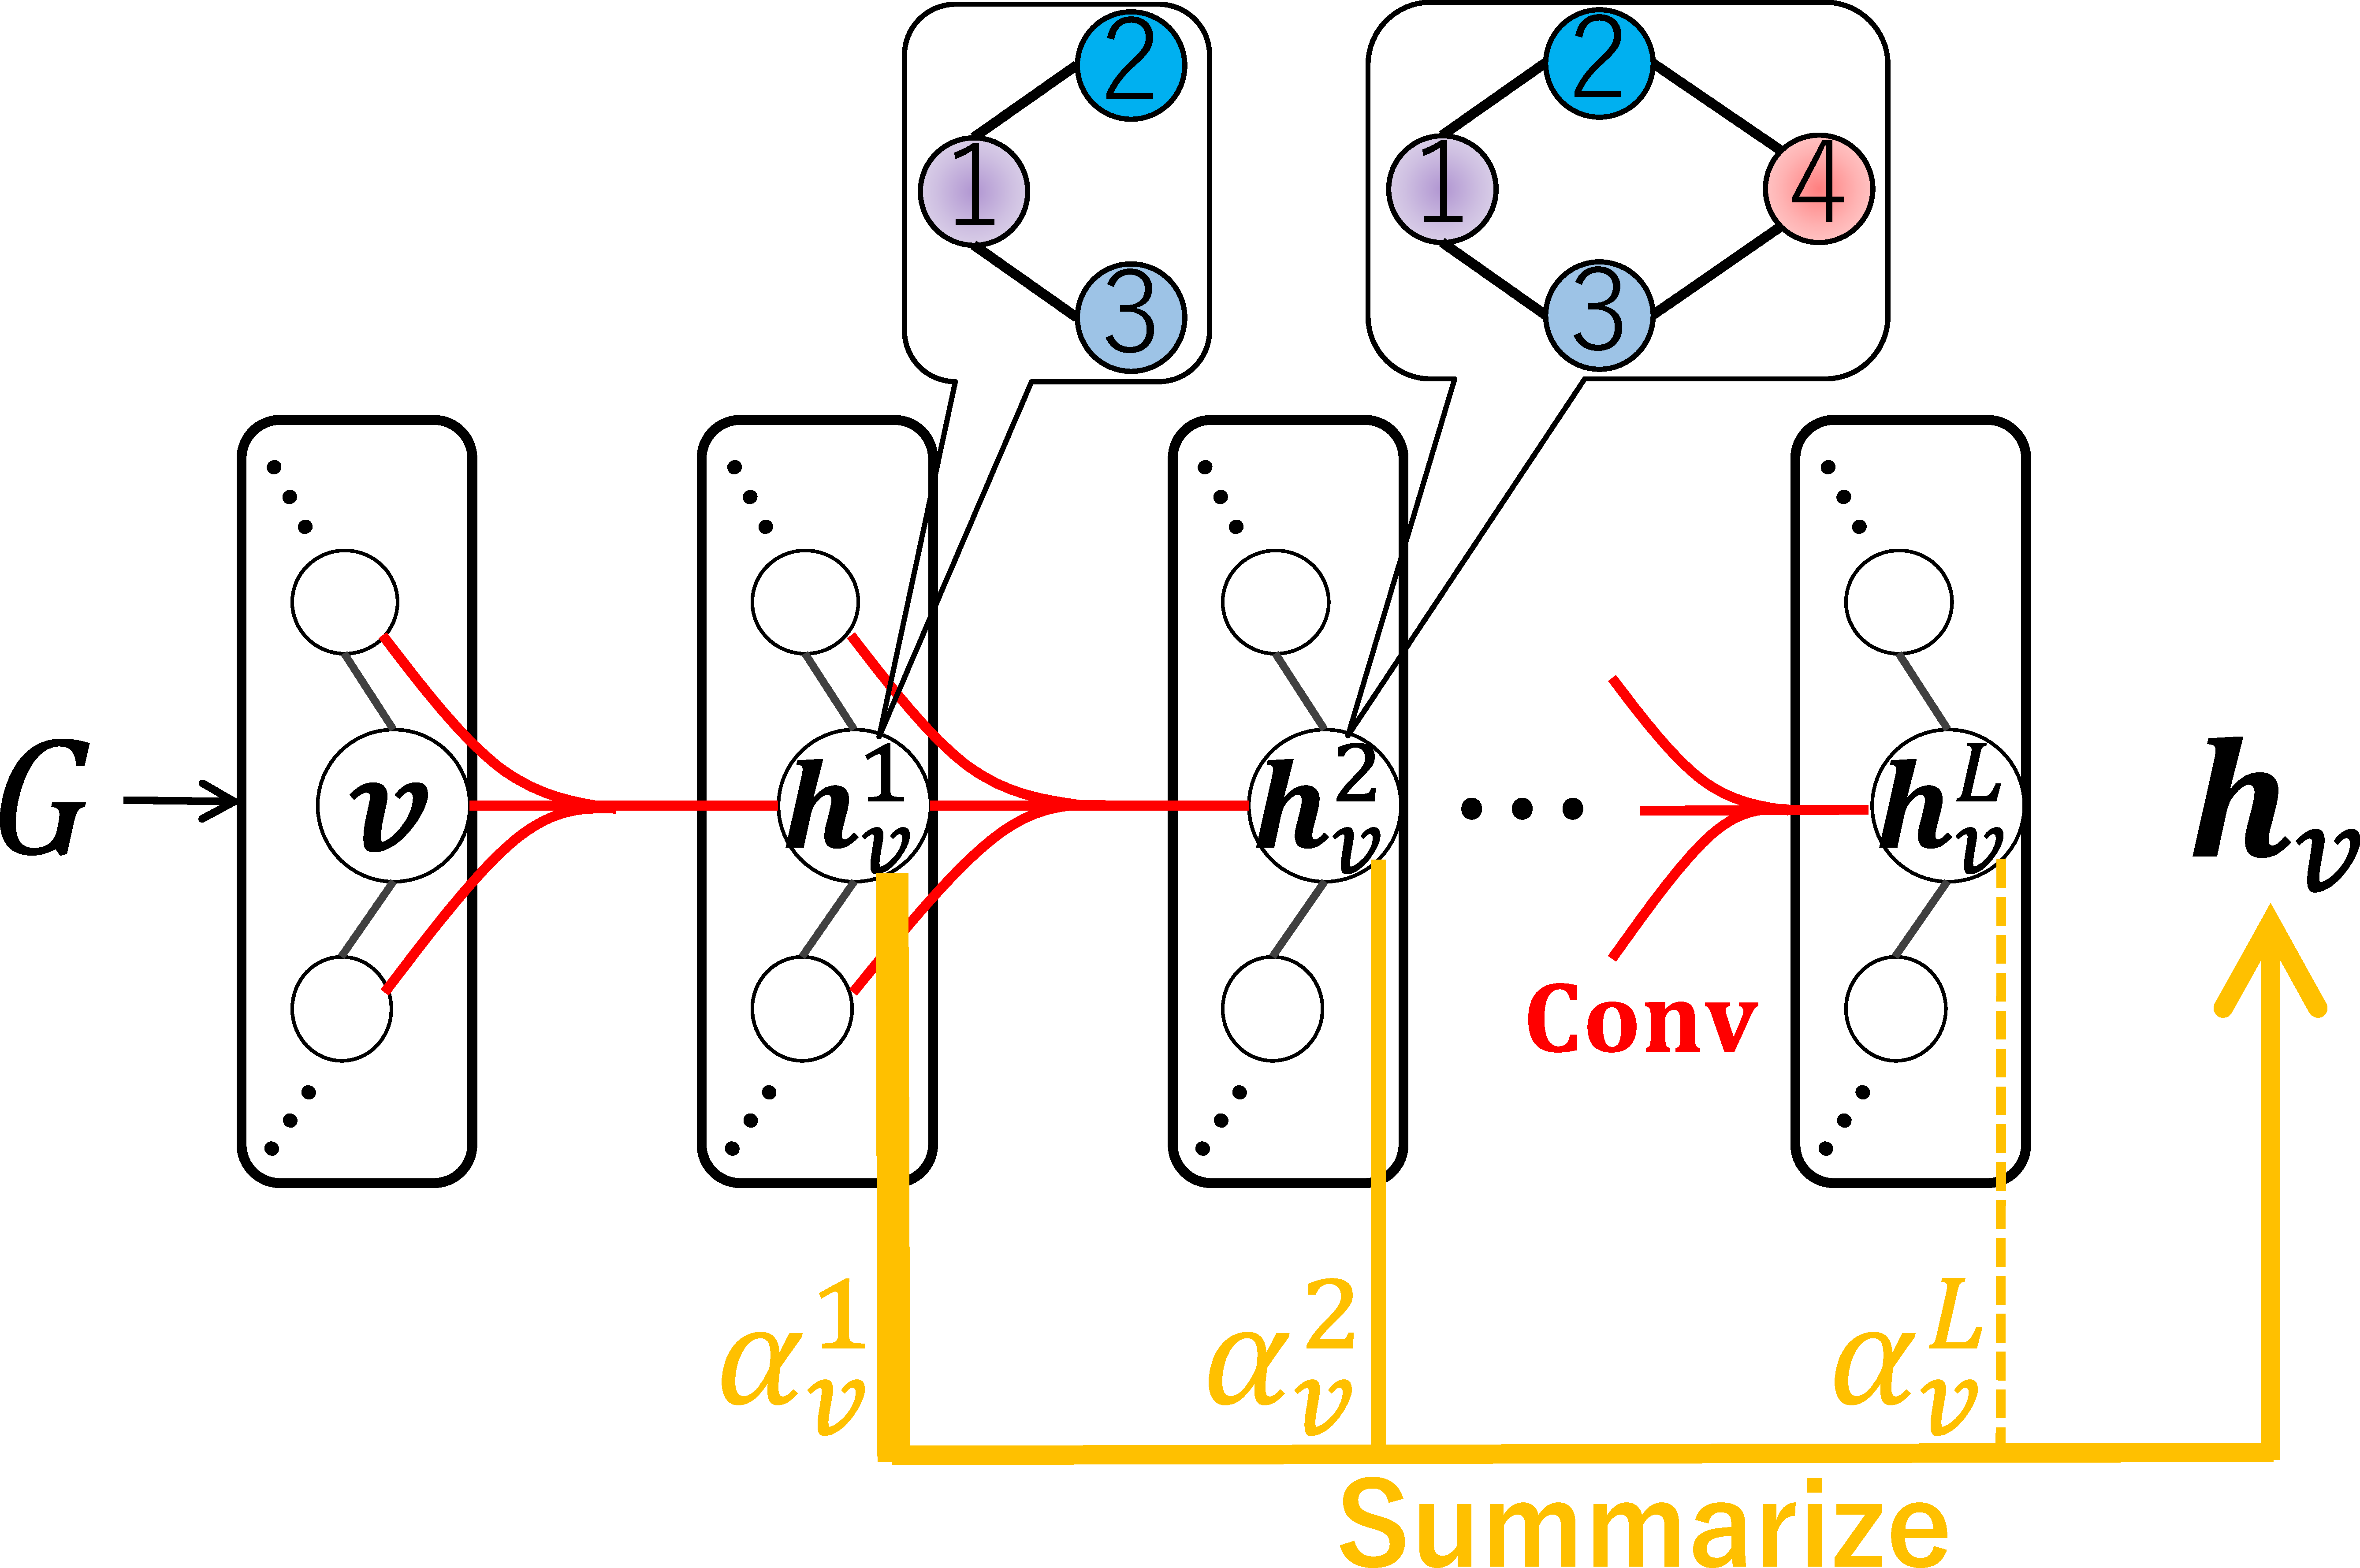
\includegraphics[height=7cm,width=9.5cm]{summarize-gnn.pdf}
  \vspace{-6mm}
  \caption{Summarize-GNN(図\ref{fig_example}の例のグラフ$G$を入力した場合)}
  \label{fig_summarize_gnn}
\end{figure}

%%%%%%%%%%%%%%%%%%%%%%%%%%%%%%%%%%%%%%%%
\section{評価実験}
\label{sec_experiment}

\begin{table}[!h]
  \begin{minipage}[!h]{.23\textwidth}
    \begin{center}
      \begin{tabular}{|l|l|l|}
        \hline
        \multicolumn{1}{|c|}{} & \multicolumn{1}{c|}{$L=2$} & \multicolumn{1}{c|}{$L=8$} \\ \hline
        GNN                    & 89.0                       & 76.8                       \\ \hline
        Skip-GNN               & 89.0                       & 86.8                       \\ \hline
        CS-GNN                 & 89.3                       & 88.8                       \\ \hline
        SS-GNN                 & 89.6                       & 89.4                       \\ \hline
      \end{tabular}
    \end{center}
    \caption{左側の表の見出し}
    \label{左側の表のラベル}
  \end{minipage}
  %
  \hfill
  %
  \begin{minipage}[!h]{.23\textwidth}
    \begin{center}
      \begin{tabular}{|l|l|l|}
        \hline
        \multicolumn{1}{|c|}{} & \multicolumn{1}{c|}{$L=2$} & \multicolumn{1}{c|}{$L=8$} \\ \hline
        GNN                    & 89.0                       & 76.8                       \\ \hline
        Skip-GNN               & 89.0                       & 86.8                       \\ \hline
        CS-GNN                 & 89.3                       & 88.8                       \\ \hline
        SS-GNN                 & 89.6                       & 89.4                       \\ \hline
      \end{tabular}
    \end{center}
    \caption{右側の表の見出し}
    \label{右側の表のラベル}
  \end{minipage}
\end{table}

%%%%%%%%%%%%%%%%%%%%%%%%%%%%%%%%%%%%%%%%
\section{まとめ}

%%%%%%%%%%%%%%%%%%%%%%%%%%%%%%%%%%%%%%%%

\bibliographystyle{jplain}
\renewcommand{\bibname}{参考文献}
\begin{thebibliography}{1}
\addcontentsline{toc}{chapter}{参考文献}
\markboth{参考文献}{参考文献}
\vspace{-2mm}

\bibitem{Kipf}
T. N. Kipf, M. Welling.:
Semi-supervised classification with graph convolutional networks,
{\it arXiv Preprint}, arXiv:1609.02907 (2016).
\vspace{-0.3mm}

\bibitem{Xu1}
K. Xu, et al.:
Representation learning on graphs with jumping knowledge networks,
{\it ICML}, pp.~5453--5462. PMLR (2018).
\vspace{-0.3mm}

\bibitem{Vaswani}
A. Vaswani, et al.:
Attention is all you need,
{\it NIPS}, pp.~5998--6008 (2017).
\vspace{-0.3mm}

\bibitem{Hochreiter}
S. Hochreiter, J. Schmidhuber.:
Long short-term memory,
{\it Neural Computation}, 9.8: pp.~1735--1780 (1997).
\vspace{-0.3mm}

\bibitem{Kim}
D. Kim, A. H. Oh.:
How to find your friendly neighborhood: Graph attention design with self-supervision,
{\it ICLR}, (2020).
\vspace{-0.3mm}

\end{thebibliography}
\end{document}